%\documentclass[aps,pra,reprint,longbibliography]{revtex4-1}
\documentclass[twocolumn]{article}

\usepackage{geometry}
\geometry{textwidth = 18cm,textheight = 24cm}

%\usepackage{multicol}
\usepackage{cite}
\usepackage{caption}
\usepackage{graphicx}
\usepackage{amsmath}
\usepackage{float}
%\usepackage{amssymb}
\usepackage{textcomp}
\usepackage{lmodern}
\newenvironment{figure_alt}
  {\par\medskip\noindent\minipage{\linewidth}}
  {\endminipage\par\medskip}

\begin{document}
	
	%-------------------- begin header -------------------%
	\centerline{\LARGE Optoelectronic Intelligence}%Light in neural systems%Intelligent optoelectronic systems
	\vspace{0.75em}
	\centerline{\Large Jeffrey M. Shainline}
	%\vspace{0.75em}
	%\centerline{\large National Institute of Standards and Technology}
	\vspace{0.5em}
	\centerline{\large NIST, Boulder, CO, 80305}
	\vspace{0.5em}
	\centerline{\large \today}
	%-------------------- end header ---------------------%
	
\begin{abstract}
To design and construct hardware for general intelligence, we must consider principles of both neuroscience and very-large-scale integration. We argue that for large neural systems capable of general intelligence, the strengths of photonics for communication and electronics for computation are complementary and interdependent. Based on these considerations, we sketch a concept for optoelectronic hardware, beginning with synaptic circuits and extending to systems at the scale of the human brain and beyond.
\end{abstract}

\section{\label{sec:introduction}Introduction}
Light is excellent for communication. Fiber optic links carry vast quantities of information across continents and between data centers. An important question in modern computing is: what is the shortest distance over which photonic communication will displace electronic interconnects? Optical links between racks in data centers are becoming common. Major companies are making big investments in photonics in the package. Monolithic optical links between a processor and memory have been fabricated in a 45-nm CMOS node with no in-line changes. Such optoelectronic systems have been demonstrated in operation \cite{suwa2015}, with significant functionality still to be explored in this zero-change approach to optoelectronic integration \cite{stra2018}. A primary challenge affecting further chip-scale electronic-photonic integration is the difficulty of achieving a light source on silicon that is robust, efficient, and economical.

In parallel with hardware considerations affecting optoelectronic integration are questions related to architecture. A prominent theme emerging since clock speed leveled off in the early 2000s is parallelism. Computation is increasingly distributed among more processor cores. Many-core architectures continue to expand into on-chip networks, in some cases resulting in highly distributed, brain-inspired systems \cite{bo2000,pfgr2013,mear2014,fuga2014,payu2017,dasr2018}. As compute grows more distributed, communication across interconnection networks becomes a bottleneck. The demand for energy-efficient communication bandwidth has been a major driver of on-chip photonics.

The major drivers for brain-inspired computers fall on a spectrum: energy and algorithmic efficiency for mobile applications reside on one side of the spectrum, and artificial general intelligence (AGI) resides on the other. Knowledge gained from neuroscience informs us that systems with general intelligence will benefit from very large numbers of complex computational elements as well as extreme communication between them. It is our perspective that hardware incorporating light for communication between electronic computational elements combined with an architecture of distributed optoelectronic spiking neurons will provide tremendous potential for AGI. While much of the aforementioned computing infrastructure has evolved to implement a von Neumann architecture perfoming sequential operations in the model of a Turing machine, the functioning of neural systems departs considerably from this model. Light has even more to offer in a neural computing context, and the hardware requirements are somewhat distinct from integrated photonics for digital logic. Considerations pertinent to the realization of optoelectronic hardware for AGI are the subject of this article. %The philosophy we advocate is to think first about what operations are required for intelligence at device, circuit, and system levels, and to think second about which hardware is most capable of performing these operations. 

\section{\label{sec:sructureAndFunction}Structure and function across space and time}
\begin{figure*} 
    \centering{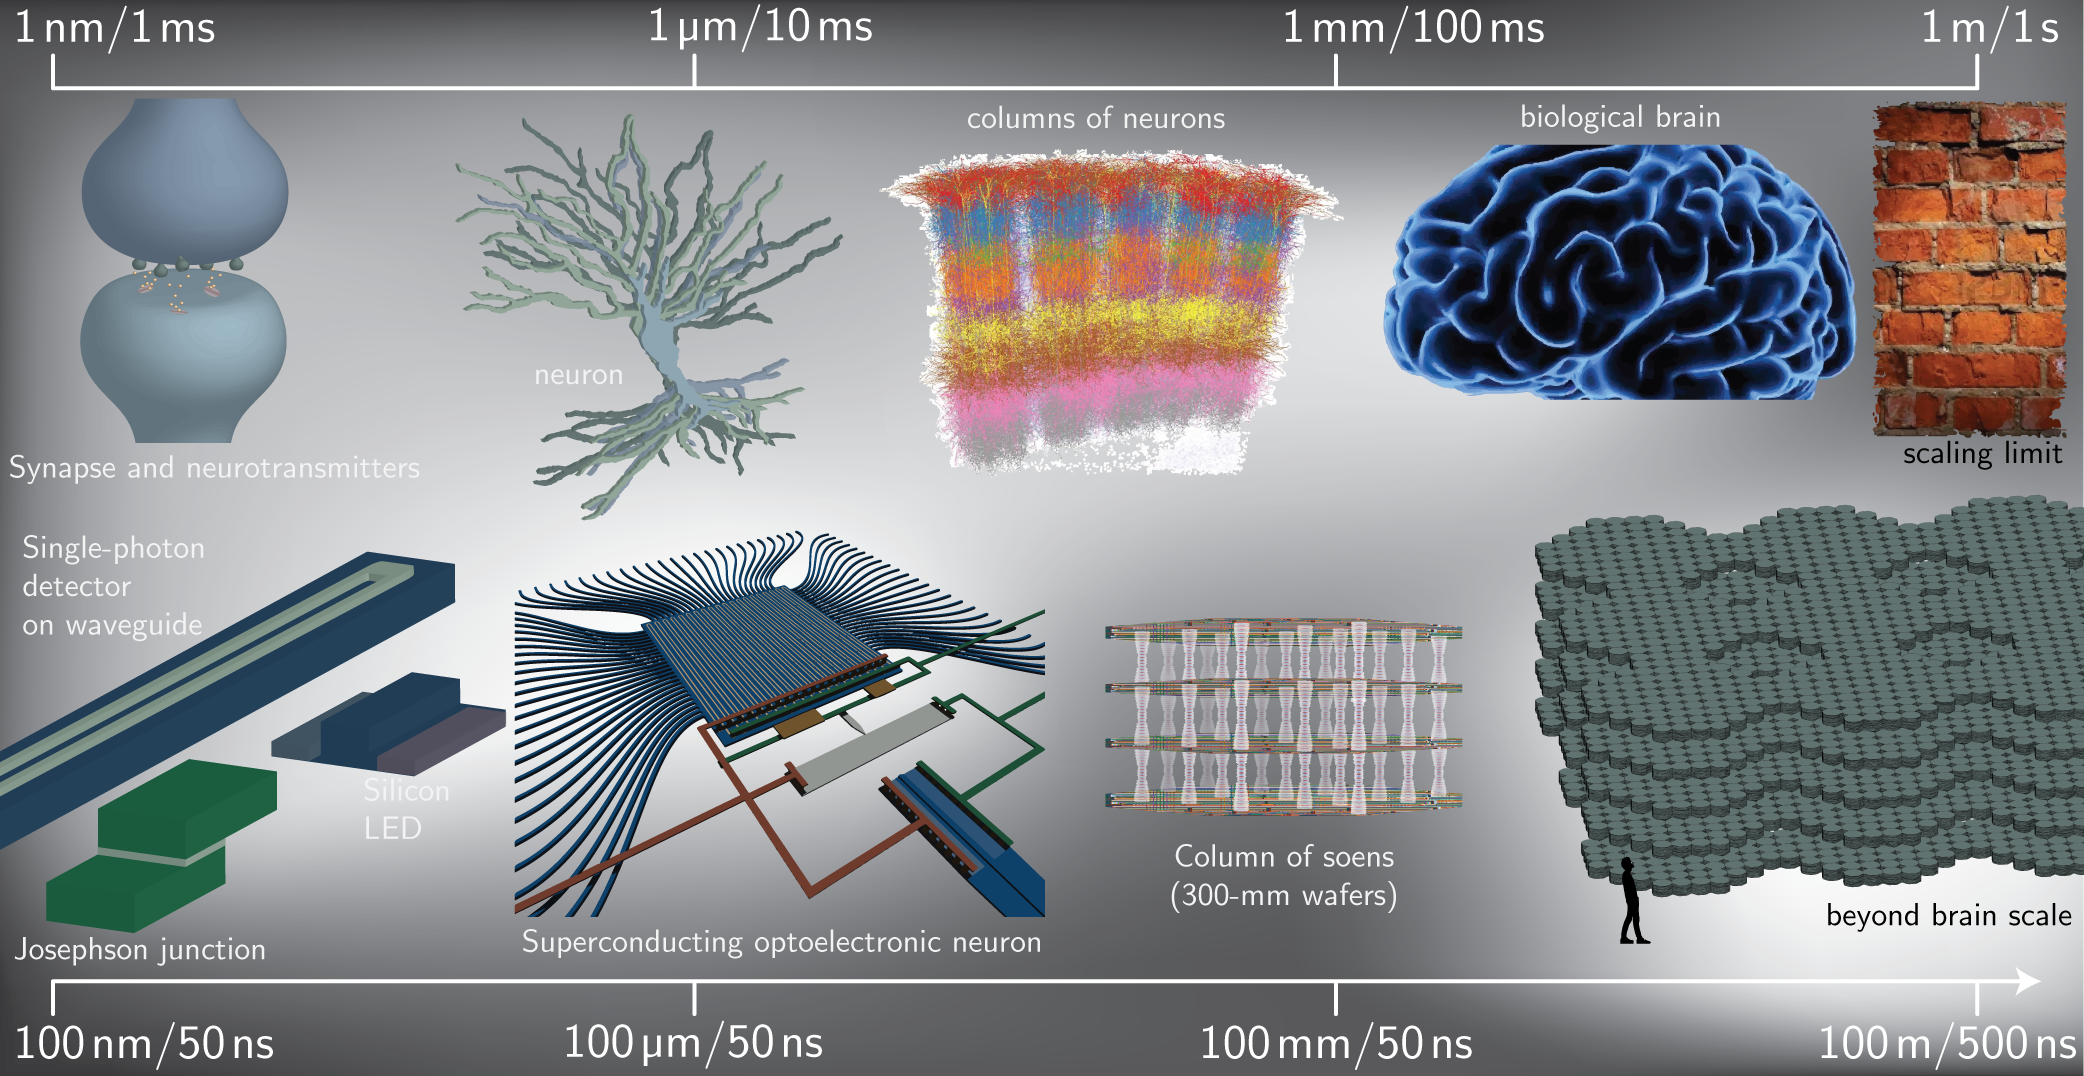
\includegraphics[width=17.6cm]{complexity_across_scales.png}}
	\captionof{figure}{\label{fig:complexityAcrossScales}Complexity across scales. Biological systems have functional components on the nanometer scale up to the full brain (roughly 0.3\,m linear dimension for full human cerebral cortex \cite{scva2014}). The speeds of the various operations are limited by chemical diffusion and axon propagation, which may ultimately limit the size of biological neural systems \cite{bu2006,shICRC2018}. By contrast, optoelectronic devices rarely have functional components with critical dimension smaller than 100\,nm, but the high speed of devices and communication enables optoelectronic systems to extend far beyond the limits imposed by the slow conduction velocity of axons.}
\end{figure*}
To guide the design of hardware for AGI, we must consider operation across spatial and temporal scales \cite{beba2016}. In Fig.\,\ref{fig:complexityAcrossScales}, we chart the structures present on various length scales and temporal scales for biological and optoelectronic hardware. The human brain has features spanning roughly eight orders of magnitude in size, from a nanometer to a tenth of a meter. Across time, activity ranges from the 1\,ms time scale of of neurotransmitter diffusion across a synapse, through the 200\,ms time scale of brain-wide theta oscillations, up to the memory retention time of the organism. The speed of devices and communication in the brain is limited by the chemical nature of various operations. The speed of synapses determines the temporal scale at which correlations can be resolved. The maximum size of the brain is limited by the slow conduction velocity of ionic signals along axons \cite{bu2006,shICRC2018}. If the brain were larger, signals would not have time to propagate between different regions during the period of theta oscillations, the network activity cycles responsible for system-wide information integration \cite{bu2006}. 

There are currently multiple efforts to utilize photonics for deep learning \cite{shha2016,chsa2018} and neuromorphic computing \cite{prsh2017}. These efforts are focused on attaining relatively small-scale systems to accomplish specific computational functions\textemdash accelerators rather than cognitive systems. We have proposed a specific approach we see as most conducive to large-scale implementation for AGI \cite{sh2018}. The approach combines waveguide-integrated light sources and single-photon detectors for communication with Josephson circuits for synaptic, dendritic, and neuronal computation. As illustrated in Fig.\,\ref{fig:complexityAcrossScales}, these optoelectronic networks are likely to have features as small as 100\,nm and potentially extend up to many kilometers. Neuronal inter-spike intervals can be as short as 50\,ns, while synaptic and dendritic processing occurs on the 50\,ps time scale of Josephson junctions. Figure\,\ref{fig:complexityAcrossScales} is intended to be viewed qualitatively and emphasizes that if communication bottlenecks can be removed, neural systems of extraordinary scale can be achieved.

But it is not sufficient to simply agglomerate large numbers of fast elements. Neural information processing requires extensive communication between neurons locally and globally, as well as a diversity of computational mechanisms implemented in synapses, dendrites, neurons, and populations. Information processing in neural systems employs local clusters of neurons to represent specific features, and the information from these clusters must be shared with other regions of the network to form a multifaceted representation of a complex stimulus. Structurally, this information processing is facilitated by networks with a high clustering coefficient yet also an average path length nearly as short as a random graph \cite{eskn2015}. Such graph structures are referred to as small-world networks \cite{wast1998}, and are ubiquitous throughout the brain \cite{sp2010}. To achieve small world networks, long-range connections are necessary. In a random network, near and distant connections are equally probable, so the average path length across the network is small, representing a lower limit on path length for a given number of edges connecting a given number of nodes. In Fig.\,\ref{fig:data}(a) we plot the number of edges required per node to achieve a given average path length as a function of the number of nodes in the random network \cite{frfr2004}. Consider the case of a network with one million nodes. We see from this plot that if we wish to maintain a path length of two, each node must make, on average, one thousand connections. For the case of a network with 100 million nodes, each node must make 10,000 connections. This is similar to the case of the hippocampus in the human brain, with nearly 100 million neurons, each with 10,000 or more synaptic connections \cite{bu2006}. Maintaining a short path length across the network is critical for information integration, and this appears to be a factor driving the connectivity of biological neural systems. In the present context, attaining short average path length is an important motivator in designing artificial hardware capable of comparable connectivity, which leads us to consider using light for communication.
\begin{figure} 
    \centering{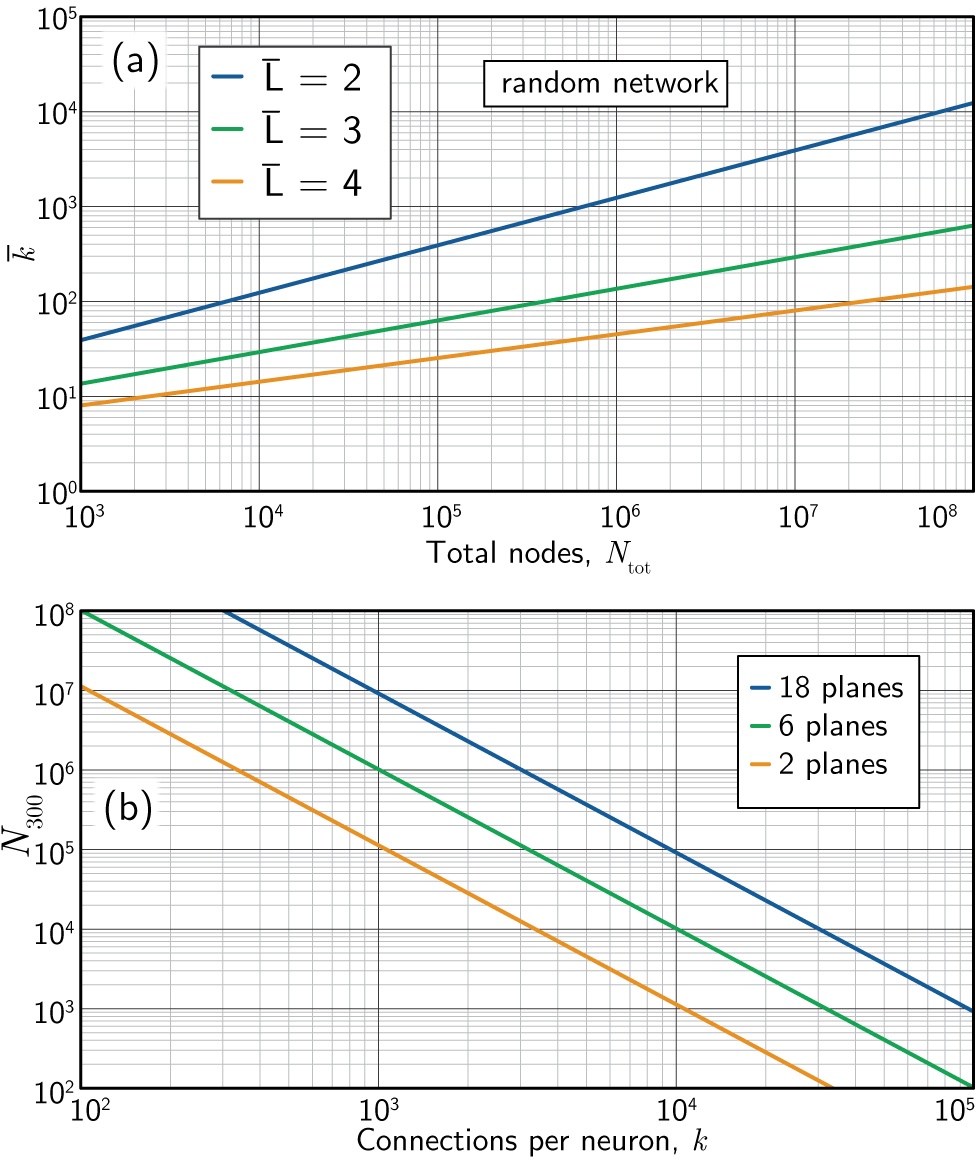
\includegraphics[width=8.6cm]{data_plots.png}}
	\captionof{figure}{\label{fig:data}Scaling considerations for optoelectronic neural systems. (a) The average number of connections per node required to maintain a give average path length across a random network as a function of the total number of nodes in the system. (b) The total number of nodes that can fit on a 300\,mm wafer as a function of the number of connections per node in the wire-limited regime \cite{ke1982}. (c) The area of the neuronal pool as a function of the frequency of neuronal oscillations assuming light-speed communication \cite{shICRC2018}.}
\end{figure}

In addition to small-world characteristics, networks of the brain demonstrate a hierarchical architecture wherein minicolumns aggregate into columns, columns into modules, and modules into complexes. This fractal property is necessary to enable networks to continue to scale arbitrarily, with dynamics constrained only by the physical hardware and spatial extent of the system rather than by the ability to communicate across the network \cite{plth2006}.  Hierarchical architecture with simple device behavior is sufficient to achieve some of the dynamical features of the brain, such as neuronal avalanches \cite{be2007,frla2013} that are observed in the resting state \cite{peth2009}. Other dynamical behaviors thought to be necessary for attention, cognition, and learning, such as cross-frequency coupling \cite{heze2010} and synaptic plasticity \cite{somi2000,mage2012,ab2008,fudr2005}, likely require complex capabilities at the device level. Dynamical synapses, dendrites, and neurons allow the same structural network to realize myriad functional networks adapting on multiple time scales. 

On the time scale of neuronal inter-spike intervals, short-term plasticity enables synapses to rapidly adapt, resulting in temporal filtering of afferent spike trains \cite{abre2004}. Also over short time scales, inhibitory neurons can silence or give voice to specific synapses, clusters of synapses on dendrites, or neurons. Over time scales long compared to an average inter-spike interval, synaptic plasticity is employed to store memories and adapt the network to a small-world architecture \cite{shki2006}. Learning in the presence of a continually changing environment while maintaining long-term memories is achieved through spike-timing-dependent plasticity (STDP) \cite{somi2000,mage2012} and metaplasticity \cite{fudr2005,ab2008}. Neurons employing inhibition \cite{budr2004}, dendritic processing \cite{haah2015,stsp2015,sava2017}, short-term \cite{abre2004}, and long-term synaptic plasticity \cite{somi2000,mage2012,ab2008,fudr2005} can make efficient use of a structural network by dynamically adapting on time scales from an inter-spike interval to the lifetime of the system. While light is excellent for communication, electrical circuits are better equipped to perform these nonlinear, dynamical functions. In particular, Josephson circuits naturally manifest many of the neuromorphic operations we seek \cite{sh2018}.

We mention these considerations of network structure and device dynamics to emphasize that neural information processing depends critically on operations best performed by light and well as on operations best performed by electronics. Neural information processing will benefit immensely from optoelectronic integration. We now discuss the proposed hardware elements in more detail.

\section{\label{sec:synapsesDendritesAndNeurons}Optoelectronic synapses, dendrites, and neurons}
We envision optoelectronic hardware with photonic communication along waveguides playing the role of axons, and computation performed in electronic synapses, dendrites, and neurons. We mentioned previously that we use single-photon communication links and Josephson circuits in this hardware. We make these choices to enable scaling to large systems. There are $10^{14}$ synapses in the human brain. An artificial system must use very low energy per synaptic event if it is going to support activity across this number of synapses with a feasible amount of power. If even 10\,nW is dissipated per synapse to retain the state, the system will use a megawatt to remember what it learned. Having chosen to communicate synaptic events with light, the quantum limit is a single photon per synaptic connection. We have designed a synapse that detects a single infrared photon and requires no power to retain the synaptic state. The synapse utilizes a superconducting-nanowire single-photon detector (SPD), a current-biased strip of superconducting wire roughly 100\,nm in width and 5\,nm in thickness. In the steady state, the current bias flows straight to ground, and upon detection of a photon, a small section of the wire is driven from the superconducting phase to the normal-metal phase, resulting in a transient resistance that diverts the current bias across a load.

In the present context, to achieve the desired synaptic operation, an SPD can be combined in circuits with Josephson junctions (JJs) and superconducting loops coupled through mutual inductors to achieve the functions needed for neural information processing. Candidate synaptic, dendritic, and neuronal circuit designs have been presented in Refs.\,\cite{sh2018,sh2018b,sh2018c,sh2018d}, and much more innovation is certainly possible. In optoelectronic synapses of this design, the current bias across a single JJ establishes the synaptic weight. This current bias can be modified through various photonic and electronic means based on control signals or network activity. Inhibition is straightforward with opposing mutual inductors. Dendritic and neuronal nonlinearities are a natural consequence of the Josephson junction critical current. Due to the prominent role of superconducting current storage loops, we refer to these as loop neurons. In the operation of loop neurons, a single photon triggers a synaptic event, and STDP is induced by two photons\textemdash one from each neuron associated with the synapse.

In addition to the choice of SPDs as the detectors in the system, we must also select a light source, which must be fabricated across wafers by the millions for economical, brain-scale systems. Because our choice of detectors dictates cryogenic operation, silicon light sources operating at 4\,K are an option \cite{da1989,shxu2007}. This neural system may be one of the few applications where silicon light sources are appropriate and sufficient. The light sources we have in mind are silicon LEDs \cite{buch2017}, employing luminescence from defect-based dipole emitters \cite{dali1987,absa2018}. From the perspective of VLSI, achievement of a silicon light source of sufficient performance would be the greatest contribution to the success of this technology. If cryogenic operation enables both single-photon detectors and silicon light sources, it will almost certainly be worth the added complexity required for cooling.

\begin{figure*} 
    \centering{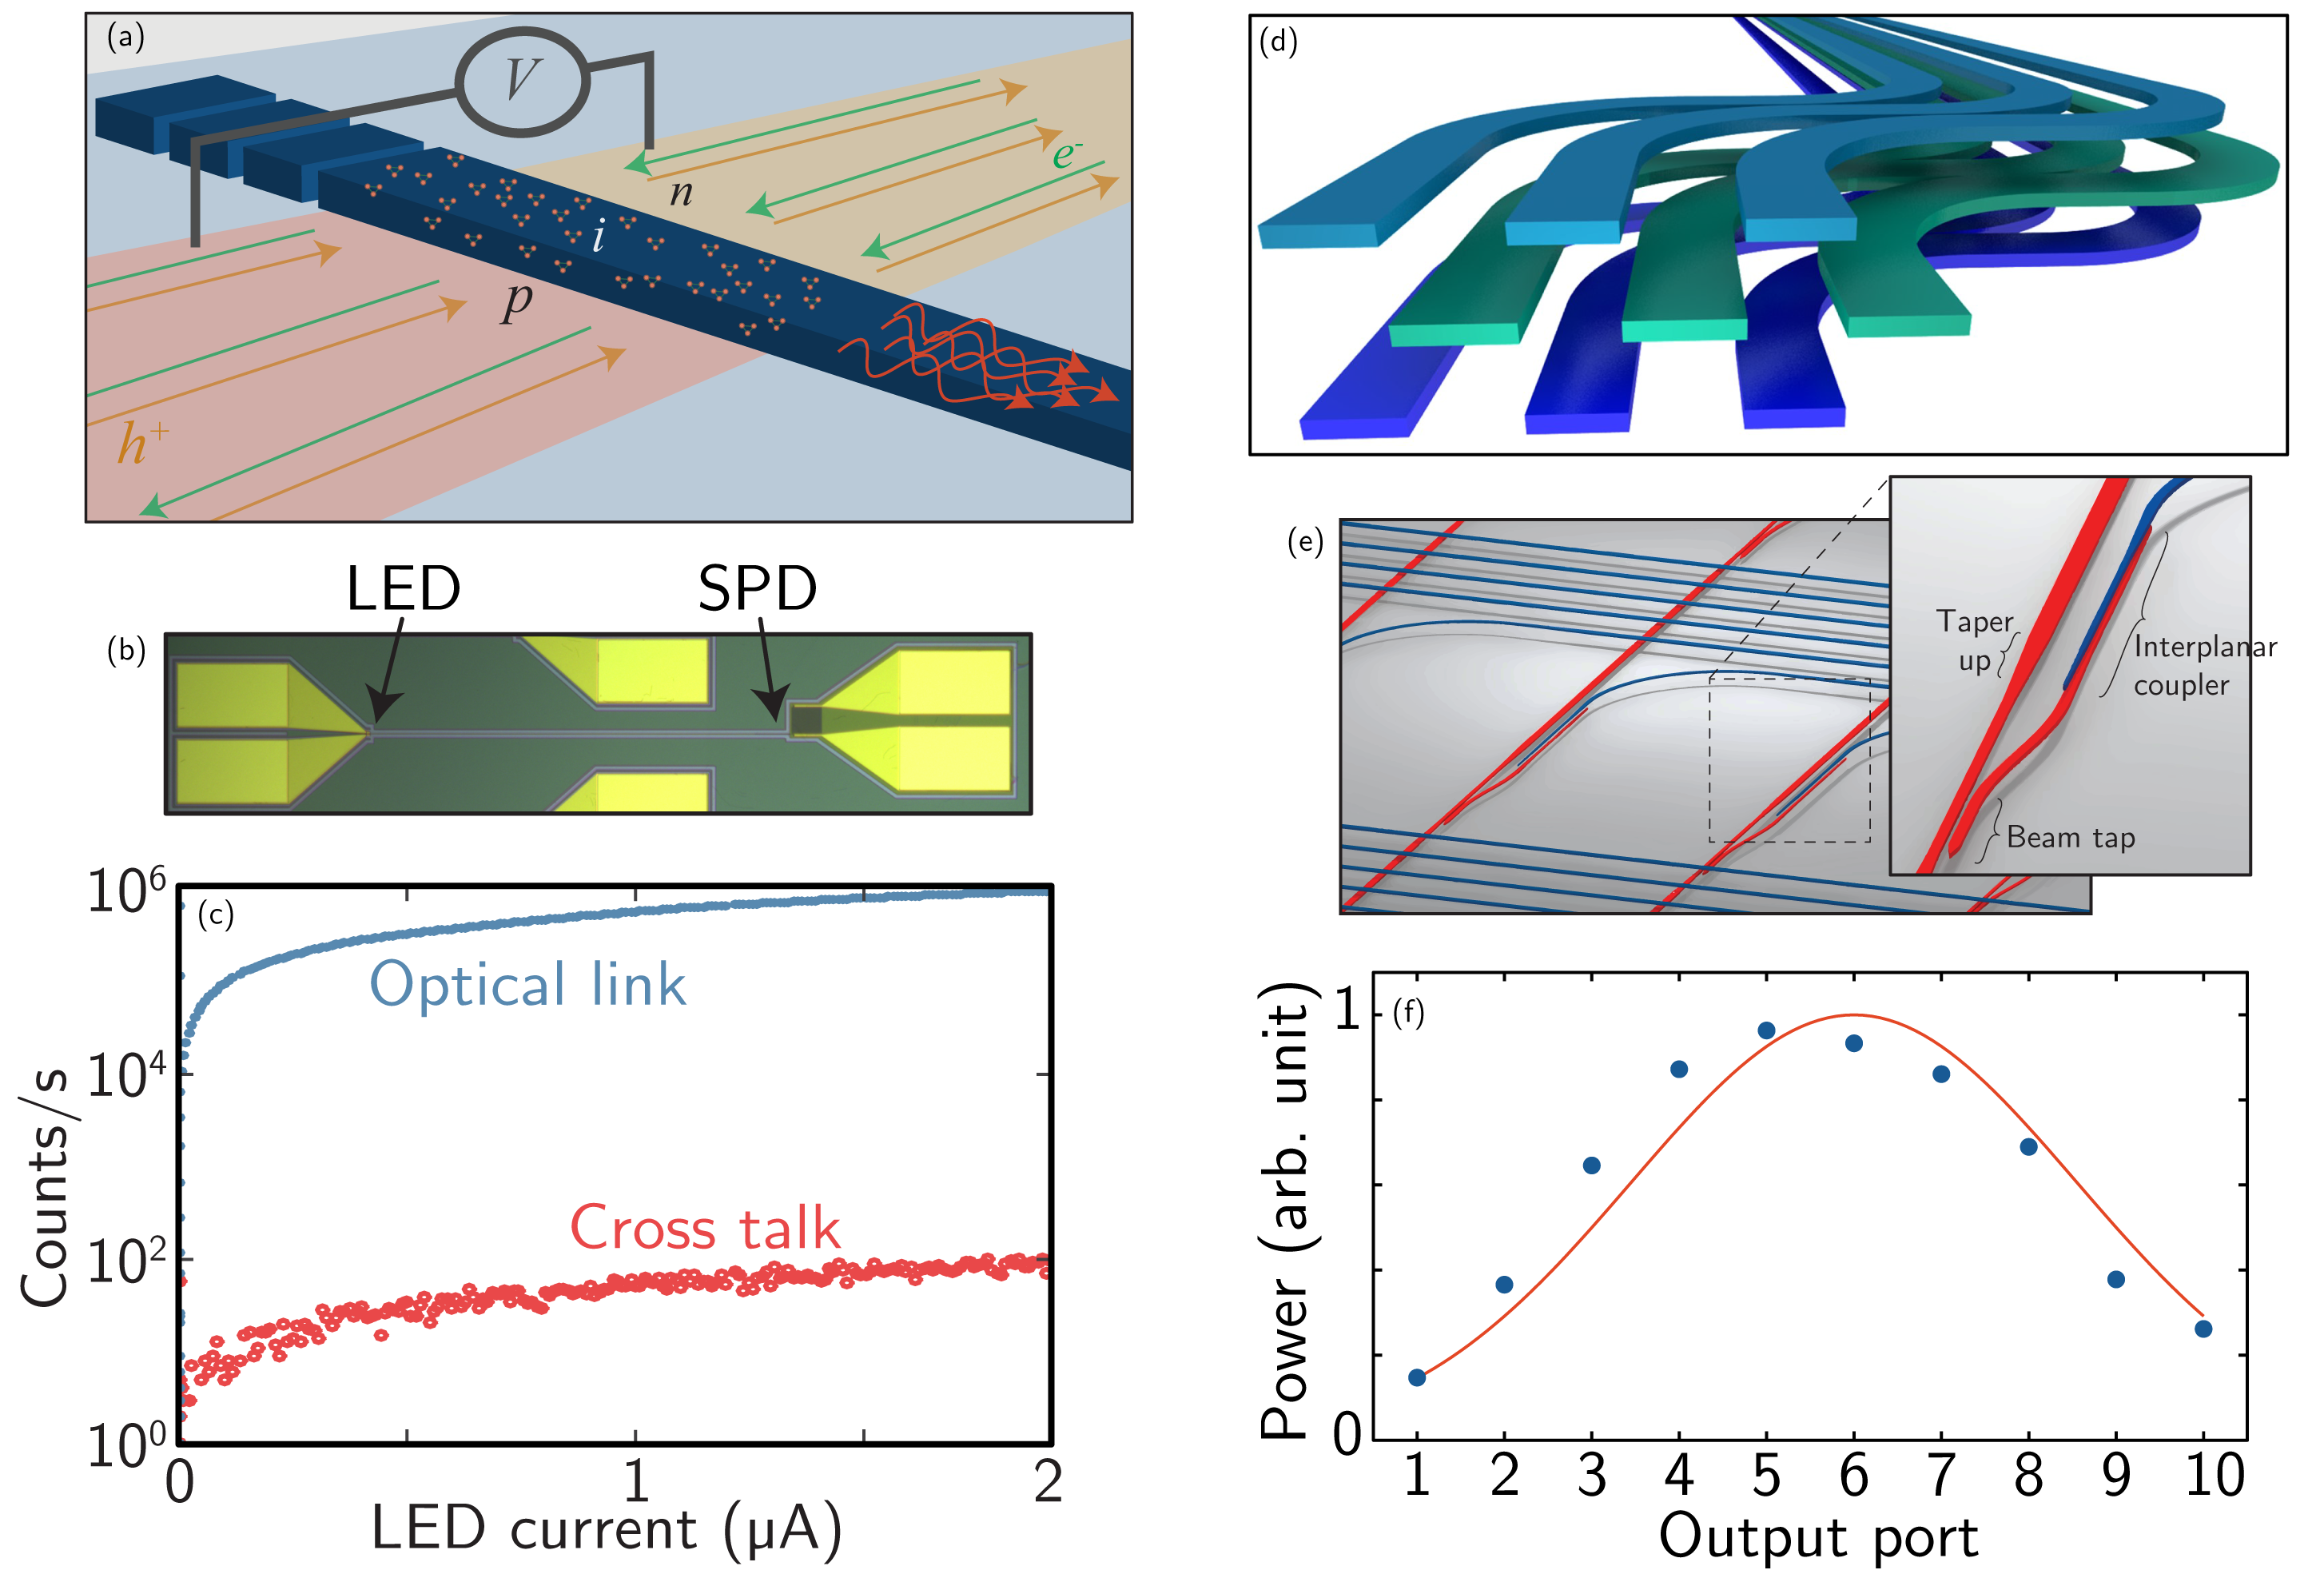
\includegraphics[width=17.2cm]{experimental.png}}
	\captionof{figure}{\label{fig:experiment}.}
\end{figure*}
To achieve complex neural circuits, we aim to combine light sources, detectors, and superconducting circuit elements. We summarize our experimental progress towards this end in Fig.\,\ref{fig:experiment}. We have demonstrated waveguide coupling of light from micron-scale all-silicon LEDs to integrated SPDs on a silicon photonic chip (Fig.\,\ref{fig:experiment}(a,b), \cite{buch2017}). The performance achieved in the first iteration of these optical links was not yet adequate. The observed efficiency was $5\times10^{-7}$, while $10^{-3}$ is desirable for achieve large systems \cite{sh2018e}. Yet the simplicity of both the source and detector made the demonstration of a monolithic optical link far easier than for room-temperature operation. For this application, high-performance light sources are unnecessary. The light sources are only required to produce incoherent pulses of 10,000 photons ($\approx 1$\,fJ) at 20\,MHz when operating at 4\,K. If silicon light sources can meet these performance specifications, the hardware stands a chance of enabling brain-scale systems with 30,000 times the speed.

We have also demonstrated superconducting amplifiers capable of generating the voltage required to produce light from a silicon diode (Fig.\,\ref{fig:experiment}(c,d), \cite{mc2019}). Generating more than a millivolt with superconducting circuits requires some effort due to the scale of the superconducting energy gap, but the thin-film, micron-scale cryotron demonstrated in Ref.\,\cite{mc2019} leverages the extreme nonlinearity of the superconducting phase transition to rapidly generate high impedance and voltage with low energy, thus driving a semiconductor light source during each neuronal firing event. The light thus produced fans out across a network of micron-scale dielectric waveguides terminating on the superconducting detectors at each synaptic connection. We have demonstrated multiple vertically integrated plains of these waveguides (Fig.\,\ref{fig:experiment}(e,f), \cite{chbu2017}), and used them to implement the architecture of a feed-forward neural network with two layers of 10 neurons per layer and all-to-all connectivity \cite{chbu2018}. These experimental demonstrations point to a much deeper pool of potential that may lie ahead.  

\section{\label{sec:communication}Communication with guided light}
A key premise of this work is that photons are excellent for communication across large-scale neural systems. To explain why we place this conjecture at the center of hardware development, we briefly summarize the physical limitations of electrical interconnection networks \cite{hepa2012}. It is impracticable in silicon electronics for a single device to source current to many other devices. A shared communication network must be employed. In contemporary computing, switched media networks are used for this purpose. Each device must then only communicate to the nearest switch in the network. Because the communication infrastructure is shared, devices must request access to the switch network to transmit messages. Arbitration must be performed, wherein devices are queued and sequentially granted access. This approach to communication between electronic devices leverages the speed of electronic circuits to compensate for the challenge of direct communication. The limitations are reached when many devices must communicate with many other devices simultaneously. Unfortunately, this is important in neural information processing. While neural activity is generally sparse, during large neuronal avalanches, or during coordinated gamma bursting, many neurons need to communicate simultaneously across the network. As more neurons, each with many synapses, are added to the network, the average frequency of neuronal firing events must decrease, and integration of information across the network is limited by the communication infrastructure.

In spite of these communication challenges, CMOS hardware is capable of significant feats of neuromorphic computing \cite{bo2000,pfgr2013,mear2014,fuga2014,payu2017}, with exciting innovation presently occurring \cite{kuwa2017,dasr2018}. Our goal in mentioning the electronic communication bottlenecks is to emphasize that the physics of light is complimentary to that of electrons. Photons, being uncharged bosons, interact very weakly with each other. Photons can co-propagate on waveguides independently of one another without wiring capacitance. A pulse of photons can fan out to many destinations without a charging penalty due to wiring. This is not to say photonic communication can address an arbitrarily large number of recipients without consequence. For each new recipient, the number of photons in a neuronal pulse must increase. As destinations get further away, more energy is dissipated to propagation loss. These realities notwithstanding, it appears feasible for devices communicating with photons to make direct connections to thousands of destinations, thereby eliminating the need for the shared communication infrastructure that is the primary impediment to achieving AGI with electrical interconnections.

Having made this claim, the burden is upon us to provide evidence of the feasibility of photonic communication in large-scale neural systems. The large wavelength of light relative to the size of electronic devices (and relative to the size of devices in the brain) causes concern for the size of optoelectronic brain-scale networks. To build confidence for the feasibility of the endeavor, we sketch a vision of how such an optoelectronic neural system may be constructed.

At the foundation of this vision is the assumption that the technology will utilize the fabrication infrastructure of silicon electronics. We conjecture that silicon photonics technology will be utilized to move light between neurons. At the wafer scale, light will be guided in multiple planes of dielectric waveguides, as discussed above, and shown schematically in Fig.\,\ref{fig:communicationAcrossScales}(a). Achieving the dense routing required to connect large numbers of neurons on a wafer will require multiple planes of waveguides \cite{chbu2017,chbu2018}, just as integrated electronics requires multiple wiring layers. We anticipate optoelectronic neural systems will utilize dielectric waveguide layers deposited in the back-end-of-line in the fabrication process, with lower layers having higher index and being utilized for local connections, and higher layers having gradually lower index with lower propagation loss used for more distant connections. 

We wish to approximate the area of such photonic interconnection networks. Following Keyes \cite{ke1982}, we approximate the area required for the waveguides entering a neuron as $A_{\mathrm{n}} = (n_{\mathrm{in}} w/k)^2$, where $n_{\mathrm{in}}$ is the number of waveguides entering the neuron (in-directed synaptic connections), $w$ is the waveguide pitch, and $k$ is the number of planes of waveguides. For tiling multi-wafer assemblies, wafers diced into octagons may be advantageous, so we take the area of a wafer to be $A_8 = 2\sqrt{2}r^2$ with $r = 150$\,mm. The number of neurons that can be supported on a 300-mm wafer is given by
\begin{equation}
\label{eq:numNeuronPerWafer}
N_8 = \frac{A_8}{A_{\mathrm{n}}} = 2\sqrt{2}r^2\left(\frac{k}{wn_{\mathrm{in}}}\right)^2.
\end{equation}
This expression is plotted in Fig.\,\ref{fig:data}(b). This estimate informs us that a 300 mm wafer with six waveguide planes can support roughly one million neurons if they each have one thousand connections. More involved analysis finds a slightly smaller number \cite{sh2018e}. As a point of comparison to electrical neural systems, Ref.\,\cite{kuwa2017} finds that through multi-layer, wafer-scale integration of logic and memory, 250 million electrical neurons could fit on a 300\,mm wafer. The trade-off is speed, as the shared communication network would limit the electrical neurons studied in Ref.\,\cite{kuwa2017} to 10\,Hz operation when 1000 synaptic connections are made per neuron. Nevertheless, the message of Fig.\,\ref{fig:data}(b) is that photonic routing results in large area consumption. An optoelectronic brain larger than that of a bumble bee will not fit on a wafer.

\begin{figure*} 
    \centering{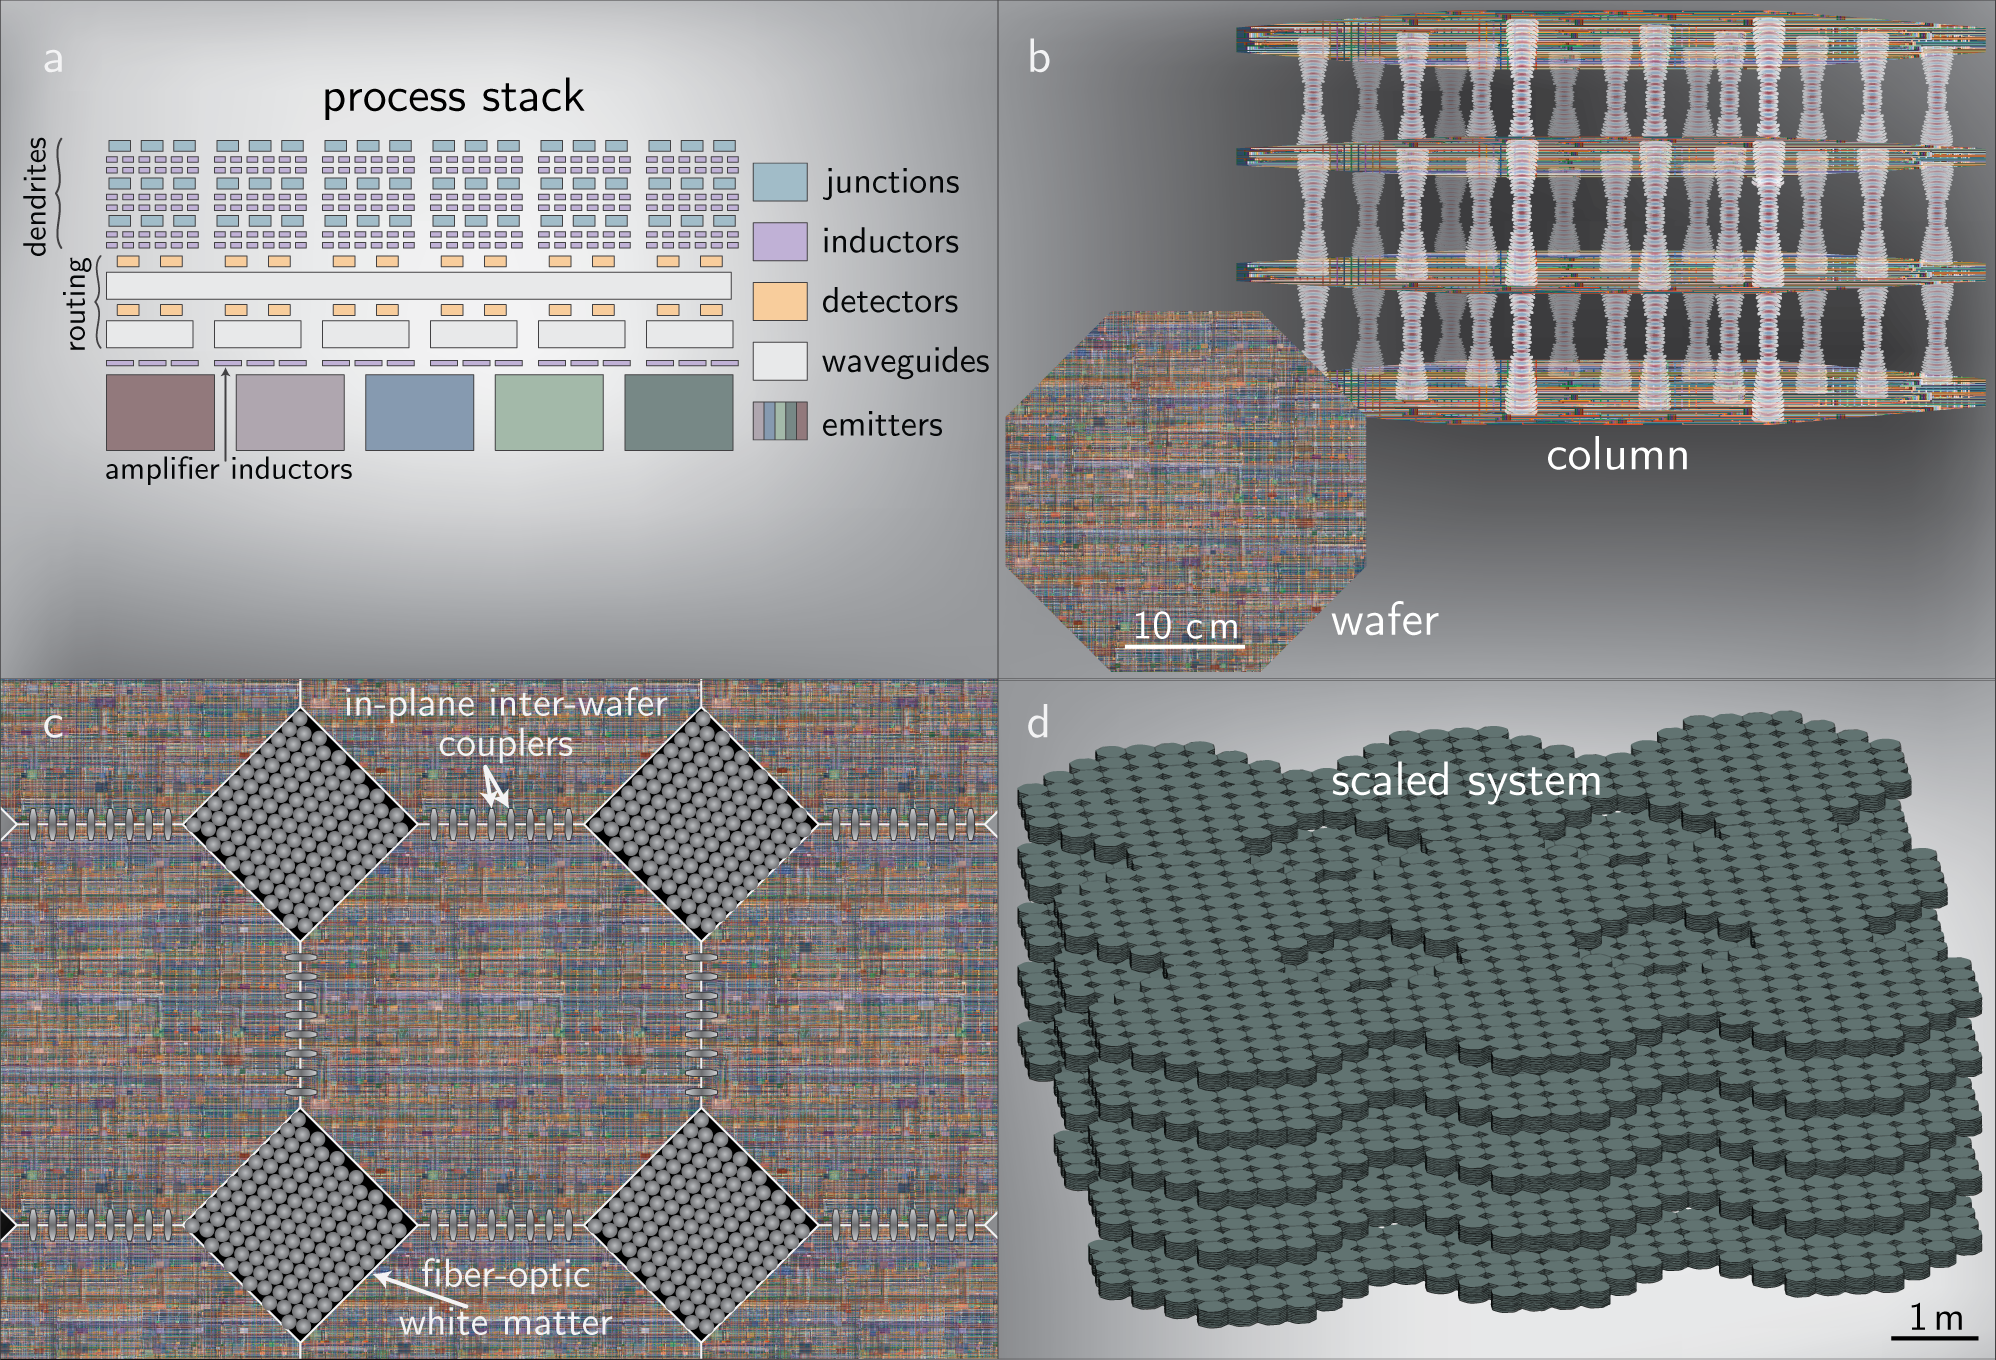
\includegraphics[width=17.6cm]{communication_across_scales.png}}
	\captionof{figure}{\label{fig:communicationAcrossScales}Schematic illustration of communication across scales in optoelectronic neural systems. (a) Schematic of a neural system implemented on a 300\,mm wafer, cut into an octagon for tiling. (b) Vertical photonic links between two stacked wafers. (c) Lateral wafer-edge links with fiber optic bundles for long-range communication. (d) A large neural system with fiber-optic connectivity between massive modules, each containing hundred to thousands of wafers.}
\end{figure*}
Optoelectronic intelligence will require communication between wafers. Wafers can be stacked vertically, and free-space optical links can send photons from a source on one wafer to a detector on a wafer above or below, as illustrated in Fig.\,\ref{fig:communicationAcrossScales}(b). Such 3D wafer-stacking techniques are being developed for electronics \cite{shhi2017,sani2018}, but the ability of light to propagate through free space (or liquid helium) and the ten-micron alignment tolerances enabled by wide-area photodetectors \cite{mave2013} make such 3D integration promising for photonic communication as well. Assuming SPDs receiving vertical communication have a pitch of 25\,\textmu m, a 300-mm octagon could support $10^8$ vertical communication links between two wafers. Considering wafers as laminar layers, as in cortex, such a configuration would result in roughly 5\% inter-layer connectivity, similar to the fraction observed in the cerebral cortex (Ref.\,\cite{bu2006}, pg. 286).

In addition to feed-forward and feed-back free-space vertical coupling, lateral inter-wafer communication can be achieved at wafer edges with in-plane waveguide couplers, as shown in Fig.\,\ref{fig:communicationAcrossScales}(c). In the octagonal tiling considered here, each wafer makes such connections to neighbors in the cardinal directions. With a 10\,\textmu m pitch, 11,500 wafer-edge couplers could be supported in each direction with 46,000 total in-plane, lateral connections. Such a system would demonstrate strong connectivity within the vertical stack of the wafers, and weaker lateral connectivity between wafers in the same horizontal plane. The reader may observe we are building toward the columnar organization of the biological cerebral cortex \cite{mo1997}.

To achieve communication from within these columns to other (perhaps distant) regions of the network, optical fibers are ideal. Within the truncated square tiling under consideration, the square areas at diagonals between wafers can support fiber-optic bundles. These optical fiber tracts are analogous to white matter in the brain. One such region could house a million single-mode fibers of 125\,\textmu m diameter. These fibers will emanate from all wafers within the column, so the number of outputs available to each wafer will depend on how many vertically integrated wafers are utilized in a column. If six wafers are stacked in a column, each wafer would have roughly 167,000 output fibers to carry information to other regions of the network. With one million neurons on a wafer, not every neuron would be able to couple to a fiber for long-distance communication. This again is consistent with brain organization wherein the number of long-distance axons emanating from a region is smaller than the number of neurons within the region. Note, however, that each of these fibers can branch as it extends through the white matter, so a neuron with access to a single wafer-edge fiber could establish multiple long-range synaptic connections. 

On a wafer, photonic fan-out across dielectric waveguides enables neurons to make thousands of direct connections without the limits of a shared switching network. Free-space and wafer-edge couplers enable significant inter-wafer communication conducive to columnar information processing. Such columns can communicate to one another locally and globally over fiber optic links. With this configuration in mind, we can assess the feasibility of constructing systems on the scale of the human cerebral cortex, with 10 billion neurons, each with thousands of synaptic connections. If a wafer holds a million neurons, a brain-scale assembly requires 10,000 wafers. Assuming the volume of white matter scales as the volume of grey matter to the 4/3 power \cite{zhse2000}, the system would fit in a volume two meters on a side\textemdash the size of a few server racks in a closet. 

\section{\label{sec:discussion}Discussion}
We are optimistic that this approach to neural information processing will be successful for physical and practical reasons. Physically, due to photonic signaling, it is possible to achieve efficient communication across the network for systems with orders of magnitude more than the 10,000 wafers comprising a brain-scale system. As we see in Fig.\,\ref{fig:data}(c), networks with activity at 20\,MHz (a conservative estimate for the ``gamma'' firing rate of loop neurons) can span an area 10 meters on a side before communication delays limit the speed of network activity. Due to superconducting electronics, the power density of such systems will be low enough for liquid helium cooling. On the practical side, fabrication of loop neurons at industrial scale appears feasible. All the proposed circuits can be created on 300\,mm wafers with existing infrastructure, such as a 45-nm CMOS node. Ten thousand wafers move through such a foundry every day. If dedicated to fabrication of optoelectronic intelligence, a single foundry may be able to produce multiple brain-scale systems per year. Assembly of the wafers into a functional system would probably not be more difficult than the construction of a contemporary supercomputer. The requirement of liquid-helium cooling is not a critical impediment.

At present, the challenge of creating an artificial intelligence comparable to a human appears formidable with the use of silicon electronics alone. The primary challenge arises because shared communication infrastructure is required, resulting in a connectivity/speed tradeoff. The use of photonic communication will mitigate this tradeoff, despite the increased size of photonic interconnection networks. Photonic fanout enables direct connections between large numbers of neurons, and the velocity of light enables communication across very large systems before communication limits network speed.% below the 20\,MHz where loop neurons are limited by superconductor reset times. 

Light is excellent for communication, while electronics excel at computation. Artificial neural hardware should be designed and constructed to leverage photonic communication while performing synaptic, dendritic, and neuronal functions with electronic circuits. Superconducting optoelectronic circuits naturally implement these functions, in part because of the utility of Josephson nonlinearities for neural computation. While neurons will pulse with as short as 50\,ns inter-spike interval, Josephson circuits will perform synaptic and dendritic computations on a 50\,ps time scale. By utilizing electronics for computation and photonics for communication, such systems could efficiently process information across a much broader range of spatial and temporal scales than the human brain. 

This hardware differs in important ways from the silicon transistors that implement Boolean logic in a von Neumann architecture. Such digital computers emerged to perform arithmetic calculations in a manner based on a Turing machine, while neural information processing departs markedly from the sequential operation of a Turing apparatus. We should not be surprised that optimal hardware may differ when objectives are so disparate. Most efforts in optoelectronic integration have focused on photonic integration with transistors for digital computing at room temperature. Due to the significance of efficient communication in neural computing, ubiquitous light sources and single-photon communication are particularly helpful. Such objectives are most straightforwardly achieved with silicon light sources and superconducting detectors. While the devices depart from conventional silicon microelectronics, the same fabrication infrastructure can be employed, thus enabling VLSI neural systems. For distant communication across the network, the low loss of fiber-optic waveguides is required. The system leverages the strengths of integrated silicon photonics as well as fiber-optic networks, semiconductor light sources and superconducting neural circuits.

What are the next steps to realize this technology? Low-cost source-detector integration at the wafer scale is required. These active devices must be augmented with improvements in deposited dielectrics for photonic routing to enable more planes of routing waveguides with lower loss. For system scaling, improved fiber-to-waveguide coupling and multi-wafer modules must be demonstrated. All the hardware improvements will not lead to AGI without further theoretical analysis at device, circuit, and system levels. Designing an architecture to achieve general intelligence is likely to be much more challenging than understanding the operation of a Turing machine. Theoretical progress is required to achieve high-performance neural systems, train them, and make them intelligent.

\bibliographystyle{unsrt}
\bibliography{optoelectronic_intelligence}
%self-organized criticality plth2006
%soc maximizes dynamic range kico2006,be2007
%power law scaling of connectivity bagr2010
%power-law power-spectral density budr2004


\end{document}